\documentclass[a4paper, 12pt, final, garamond]{book}
\usepackage{cours-preambule}

\raggedbottom

\makeatletter
\renewcommand{\@chapapp}{\'Electrocin\'etique -- chapitre}
\makeatother

\begin{document}
\setcounter{chapter}{6}

\chapter{TD~: filtrage lin\'eaire}

\section{Filtrage et spectres}

Un signal périodique $e(t)$ (de fréquence \SI{1}{kHz}), dont le spectre est
donné en figure 1, est envoyé à l'entrée de trois filtres différents. On
effectue l'analyse spectrale du signal de sortie pour chaque filtre, les
spectres obtenus sont donnés en figure 2, 3 et 4.

\begin{center}
    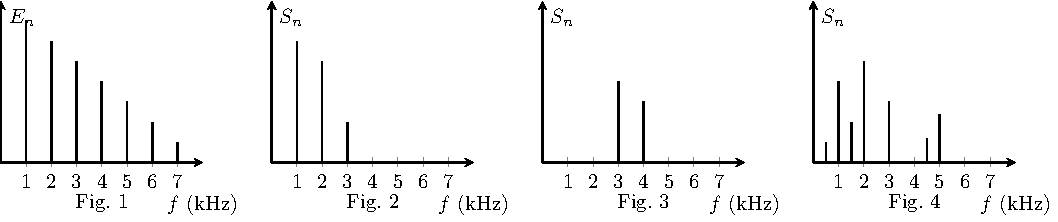
\includegraphics[width=\linewidth]{spectres_plain}
\end{center}

Quelles caractéristiques de chaque filtre peut-on déduire de ces spectres ?

\section{Filtre avec une bobine}
On considère le circuit ci-contre, avec $R = \SI{1.0}{k\Omega}$ et $L =
\SI{10}{mH}$, donnant le diagramme de \textsc{Bode} ci-dessous~:

\begin{minipage}{0.60\linewidth}
    \begin{enumerate}
        \item Sans utiliser le diagramme de \textsc{Bode}, quelle est la nature
            du filtre~?
        \item Déterminer sa fonction de transfert et l'écrire sous la forme
            \[\ul{H}(\jj\w) = H_0 \frac{\jj\dfrac{\w}{\w_c}}{1 +
            \jj\dfrac{\w}{\w_c}}\]
            avec $H_0$ et $\w_c$ des constantes à préciser.
        \item Montrer par le calcul que la pente de l'asymptote du diagramme
            de \textsc{Bode} pour $\w \ll \w_c$ est de \SI{20}{dB/décade}.
        \item On considère une tension d'entrée $u_e(t)$ somme de 3 harmoniques de
            mêmes amplitudes, de mêmes phases initiales, mais de fréquences
            respectives $f_1 = \SI{100}{Hz}$, $f_2 = \SI{1}{kHz}$ et $f_3 =
            \SI{100}{kHz}$. Donner le spectre de sortie.
    \end{enumerate}
\end{minipage}
\hfill
\begin{minipage}{0.35\linewidth}
    \begin{center}
        \hspace{10pt}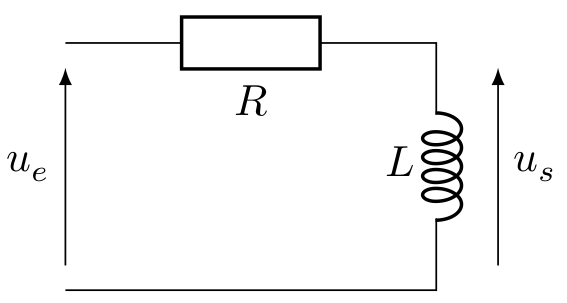
\includegraphics[width=\linewidth]{filtrebob_plain}
    \end{center}
    \begin{center}
        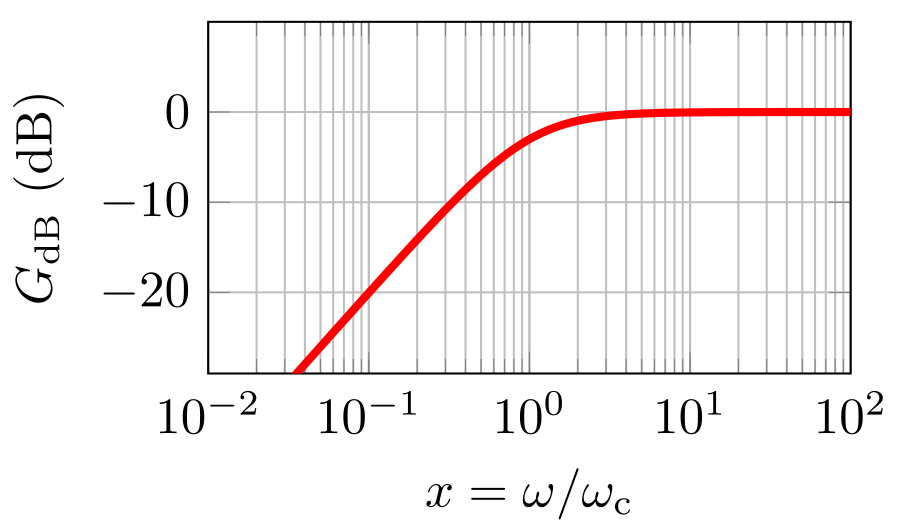
\includegraphics[width=\linewidth]{filtrebob_bode}
    \end{center}
\end{minipage}

\section{Lecture de diagrammes de \textsc{Bode}}
On donne, page suivante, les diagrammes de \textsc{Bode} de quatre filtres. Pour
chacun d'eux~:
\begin{enumerate}
    \item Indiquer le type de filtre dont il s'agit.
    \item Déterminer l'expression du signal $s(t)$ de sortie du filtre pour un
        signal d'entrée
        \[e(t) =
            E_0 +
            E_0\cos(\wt) +
            E_0\cos \left( 10\wt + \frac{\pi}{4} \right) +
            E_0\cos \left( 100\wt - \frac{\pi}{3} \right)
        \]
        avec une fréquence $f = \SI{1}{kHz}$.
\end{enumerate}
\begin{center}
    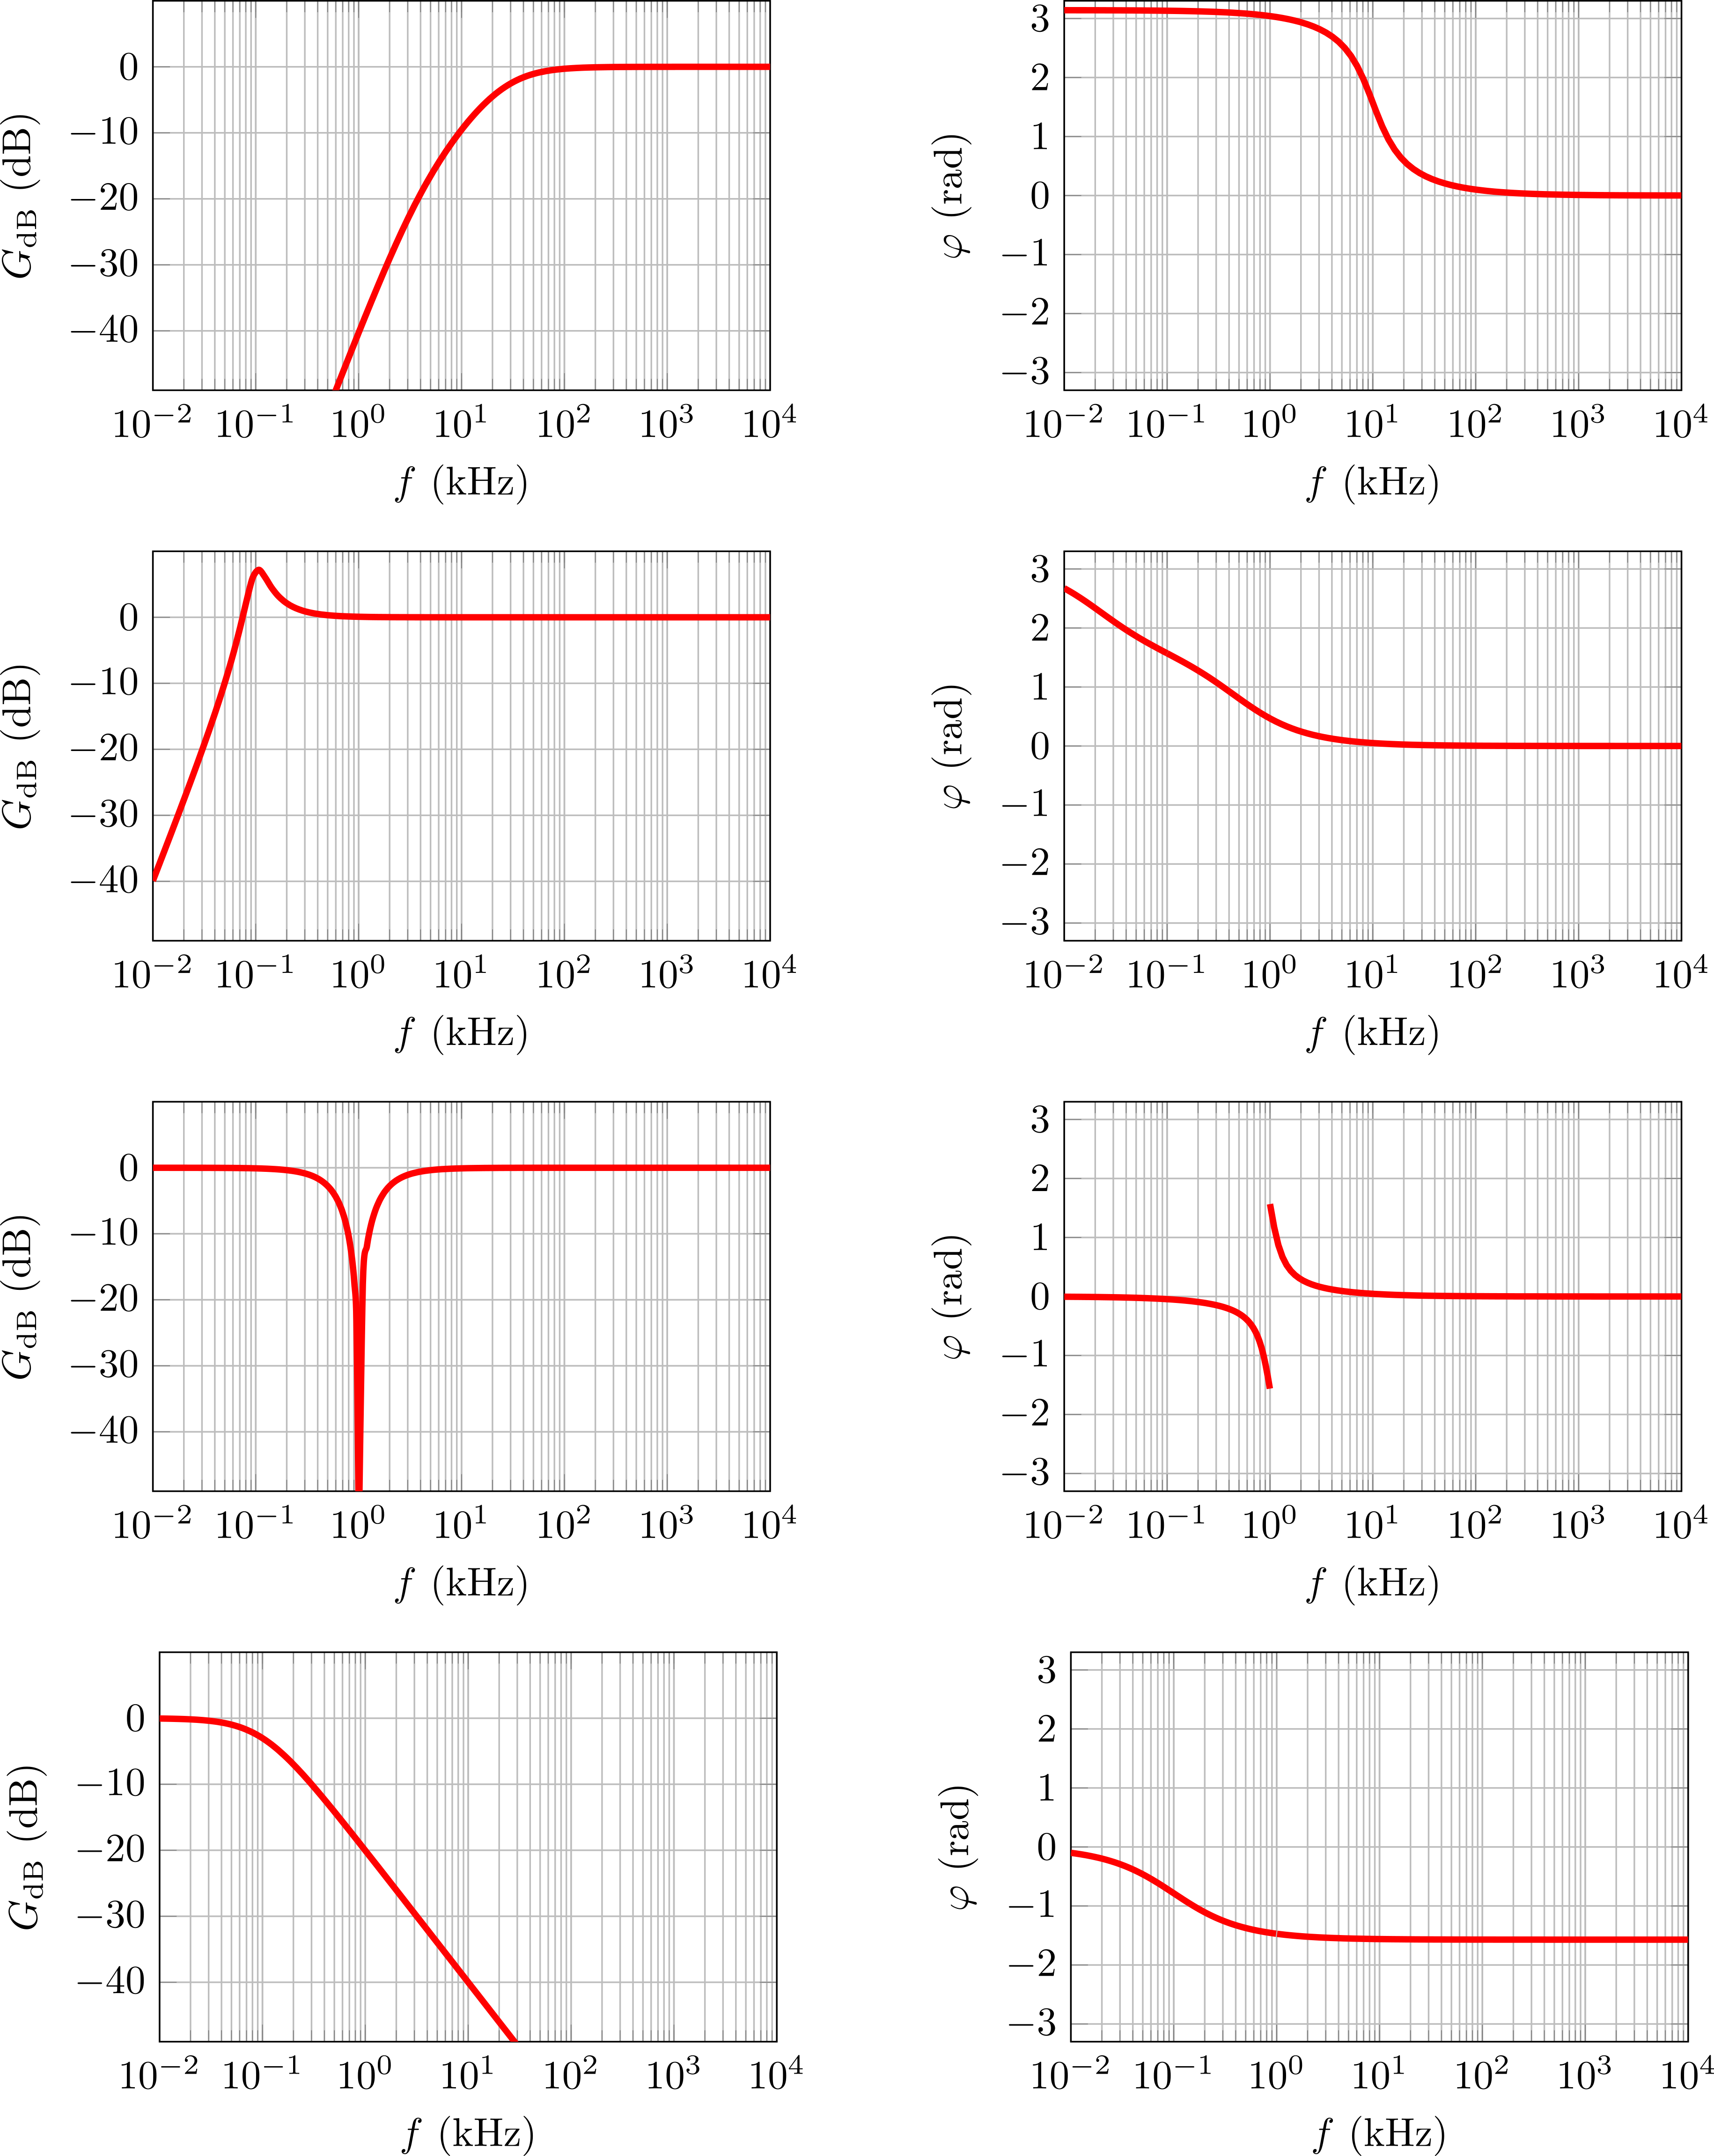
\includegraphics[scale=1]{bode_lect-plain}
\end{center}

\section{Filtre de \textsc{Wien}}
On s'intéresse au filtre de \textsc{Wien}, représenté ci-contre.
\begin{center}
    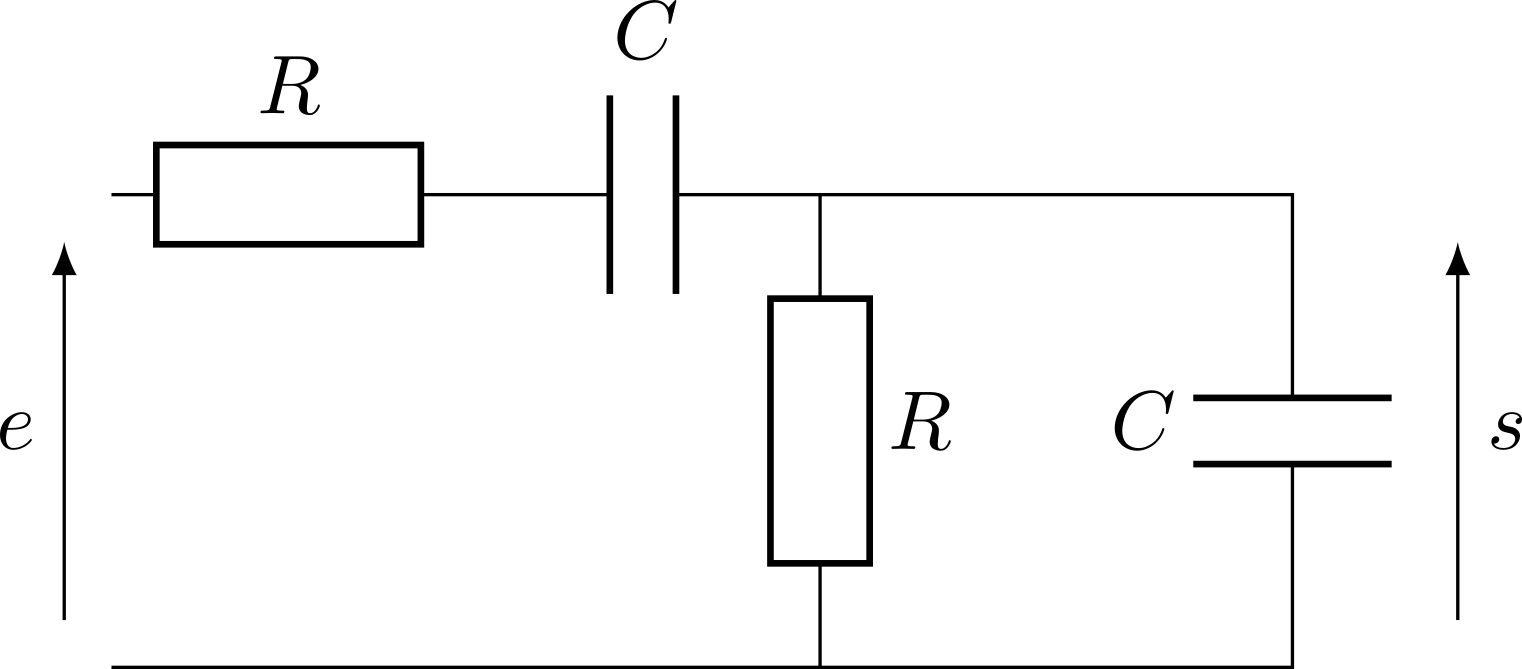
\includegraphics[width=.5\linewidth]{wien_circ-plain}
\end{center}

\begin{enumerate}
    \item Par analyse des comportements asymptotiques, déterminer le type de
        filtre dont il s'agit.
    \item Déterminer la fonction de transfert $\ul{H}$ du filtre.
    \item On pose $\w_0 = 1/RC$ et $x=\w/\w_0$. Écrire la fonction de transfert
        sous la forme
        \[ \ul{H} = \frac{H_0}{1 + \jj Q \left( x - \dfrac{1}{x} \right)}\]
        en précisant les valeurs de $H_0$ et $Q$.
    \item Calculer simplement le gain maximal du filtre, puis le gain maximal en
        décibels, et le déphasage correspondant à ce maximum.
    \item Représenter le diagramme de \textsc{Bode} asymptotique du filtre et en
        déduire qualitativement le tracé réel.
    \item Calculer la pulsation propre $\w_0$ pour $R = \SI{1.0}{k\Omega}$ et $C
        = \SI{500}{nF}$. Donner le signal de sortie du filtre si le signal
        d'entrée est
        \[e(t) = E_0 + E_0\cos(\wt) + E_0\cos(10\wt) + E_0\cos(100\wt)\]
        avec $E_0 = \SI{10}{V}$ et $\w = \SI{200}{rad.s^{-1}}$.
\end{enumerate}

\section{Filtre ADSL}
Un lutin malin semble avoir chourré votre filtre ADSL. Sale histoire.
Heureusement, vous avez les connaissances pour en recréer un~! En sachant que
les signaux transmis par une ligne téléphonique utilisent une très large gamme
de fréquences, divisée en deux parties~:
\begin{itemize}
    \item les signaux téléphoniques (transmettant la voix) utilisent les
        fréquences de 0 à \SI{4}{kHz}~;
    \item les signaux informatiques (Internet) utilisent les fréquences de
        \SI{25}{kHz} à \SI{2}{MHz}.
\end{itemize}

\begin{enumerate}
    \item Quel type de filtre faut-il utiliser pour récupérer seulement les
        signaux téléphoniques ? Les signaux informa- tiques ? Quelle fréquence
        de coupure peut-on choisir ?
\end{enumerate}
Vous réalisez le filtre ci-dessous.
\begin{center}
    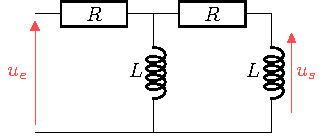
\includegraphics[width=.5\linewidth]{adsl_plain}
\end{center}

\begin{enumerate}[resume]
    \item Déterminer la nature du filtre grâce à son comportement asymptotique
        en basses fréquences et en hautes fréquences. En déduire pour quels
        signaux il peut être utilisé.
    \item Montrer que la fonction de transfert de ce filtre peut se mettre sous
        la forme~:
        \[\ul{H}(x) = \frac{-x^2}{1 + 3\jj x-x^2}
            \qavec
            x = \frac{\w}{\w_0}
        \]
        et exprimer $\w_0$ en fonction de $R$ et $L$.
    \item Tracer le diagramme de Bode asymptotique (gain et phase) de ce filtre,
        puis esquisser l'allure de la courbe réelle de gain en la justifiant.
    \item Vous possédez des résistances de $\SI{100}{\Omega}$. Quelle valeur
        d'inductance $L$ choisir pour réaliser le filtre souhaité~?
\end{enumerate}

\section{Filtre de \textsc{Colpitts}}

\begin{minipage}{.50\linewidth}
    On considère le quadripôle suivant, où $C$ est une capacité, $R$ une
    résistance et $L$ une inductance. Il est utilisé en régime sinusoïdal forcé
    de pulsation $\w$, en sortie «~ouverte~» (rien n'est branché aux bornes de
    sortie).
\end{minipage}
\begin{minipage}{0.50\linewidth}
    \begin{center}
        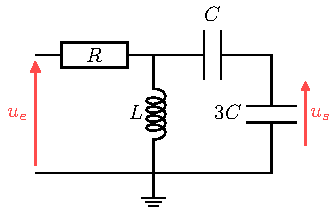
\includegraphics[width=.8\linewidth]{colpitts_plain}
    \end{center}
\end{minipage}
\begin{enumerate}
    \item Étudier qualitativement le comportement de ce quadripôle en hautes et
        basses fréquences. De quel type de filtre s'agit-il~?
    \item Déterminer la fonction de transfert $\ul{H}(\jj\w) =
        \dfrac{\ul{u_s}}{\ul{u_e}}$ et la mettre sous l'une des formes
        équivalentes~:
        \[\ul{H}(\jj\w) = \frac{A}{1+\jj Q \left( \dfrac{\w}{\w_0} -
            \dfrac{\w_0}{\w} \right)} = \frac{\jj\dfrac{A}{Q}\dfrac{\w}{\w_0}}{1
    - \dfrac{\w^2}{\w_0{}^2} + \dfrac{\jj}{Q} \dfrac{\w}{\w_0}}\]
        En introduisant des constantes $A$, $w_0$ et $Q$ dont on précisera les
        expressions en fonction de $R$, $L$ et $C$.
    \item Le diagramme de \textsc{Bode} de ce quadripôle pour $Q = 6$ est donné
        ci-dessous. Justifier l'allure des parties rectilignes du diagramme.
        Déduire du diagramme la valeur de la fréquence d'accord $f_0 =
        \w_0/2\pi$ ainsi que des fréquences de coupure.
\end{enumerate}
\begin{center}
    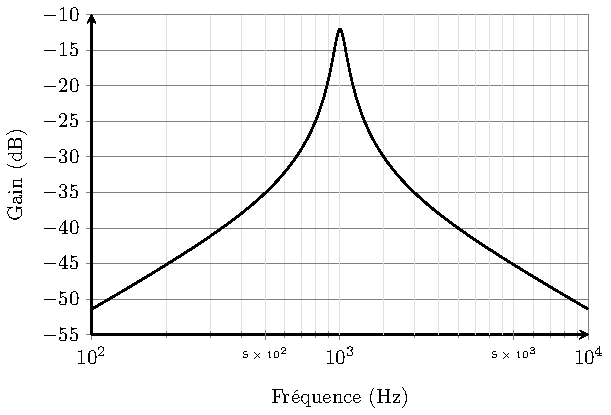
\includegraphics[width=.46\linewidth]{colpitts_bode-gain}
    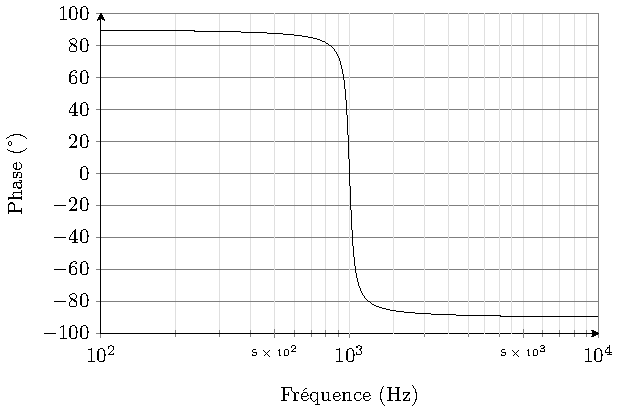
\includegraphics[width=.46\linewidth]{colpitts_bode-phase}
\end{center}

\section{Filtre de \textsc{Butterworth} d'ordre 3}
On veut réaliser un filtre de \textsc{Butterworth} d'ordre 3, dont le module $H$
de sa fonction de transfert harmonique en tension $\ul{H}$ s'exprime~:
\[H = \abs{\ul{H}} = \sqrt{\frac{1}{1+\left(\dfrac{\w}{\w_0}\right)^6}} =
    \sqrt{\frac{1}{1+x^6}}
    \qavec
    x = \frac{\w}{\w_0}
\]
\begin{enumerate}
    \item Montrer qu'une fonction de transfert $\ul{H} = \DS \frac{1}{1+2\jj x +
        2(\jj x)^2 + (\jj x)^3}$ correspond bien à un filtre de
        \textsc{Butterworth} d'ordre 3.
    \item Étudier et représenter le diagramme de \textsc{Bode} asymptotique en
        amplitude de cette fonction de transfert.
    \item On considère le quadripôle ci-dessous~:
        \begin{center}
            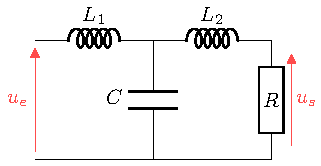
\includegraphics[width=0.5\linewidth]{butterworth_filtre-plain}
        \end{center}
        Calculer en fonction de $R$ et $\w_0$, les valeurs de $L_1$, $L_2$ et
        $C$ pour que ce filtre soit un filtre de \textsc{Butterworth} d'ordre 3.
    \item Justifier que l'on puisse réaliser le filtre de \textsc{Butterworth}
        d'ordre 3 en associant en cascade un filtre d'ordre 1 et un filtre
        d'ordre 2, comme sur le circuit suivant~:
        \begin{center}
            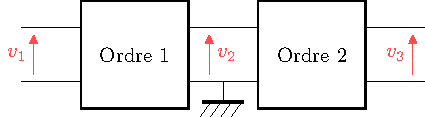
\includegraphics[width=0.6\linewidth]{butterworth_filtre_cascade-plain}
        \end{center}
        Préciser la valeur du facteur de qualité du filtre d'ordre 2.
\end{enumerate}

\end{document}
